\subsection{IMU Implementation}
Since the IMU will be connected to the ZedBoard's Pmod connector, it can be controlled by either the Programmable Logic (PL) or the Programmable Software (PS). Since the IMU's magnetometer data will be used to rotate the rangefinder data according to a compass direction, it will affect the rangefinder's step value. Since the step value is set in the PS, it is easiest to keep all of the IMU's implementation in the PS rather than take advantage of the PS-PL communication setup from Section \ref{sssec:ps_pl}. Another motivation for the PS is that the IMU data processing involves complex trigonometry. Rather than attempt this in the PL, it would be simpler to do in the PS.
\par
The Zynq7 Processing System in the PL needs to be re-customized in order to add SPI capability.

\subsubsection{Re-Customizing the Zynq7 Processing System}
The Zynq7 Processing System is easily re-customizable, as discussed in Section \ref{zynq7processingsystem}. SPI functionality can be added in the processing system's customization window under I/O Peripherals in the MIO Configuration tab. We intend to route the SPI pins to EMIO (Extended MIO) so that we could control one of the ZedBoard's PL Pmod's from the PS. Since both SPI0 and SPI1 have EMIO functionality, we arbitrarily chose SPI0 over SPI1. This process is shown in Figure \ref{enabling_spi0}.

\begin{figure}[H]
	\centerline{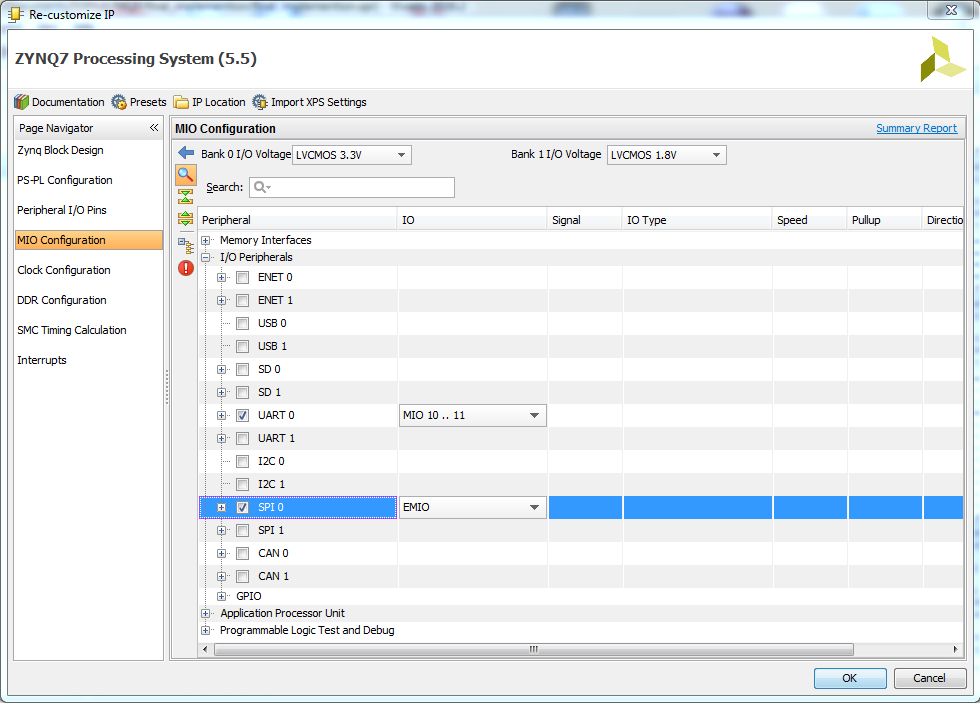
\includegraphics[width=1\textwidth]{enabling_spi0.png}}
	\caption{Re-Customizing the Zynq7 Processing System to Add SPI}
	\label{enabling_spi0}
\end{figure}


\par
talk about rerouting the SPI pins to the EMIO PMOD, differential signals?
\par
ADD NEW SECTION IF THIS ISN'T DONE IN THE PROCESSING SYSTEM CONFIGURATION
\par
This is all you brocahtoa, i got nothing.





